\section{Ziel}
In diesem Versuch sollen sowohl Zerfallskurven als auch Halbwertszeiten verschiedener radioaktiver Isotope
bestimmt werden.

\section{Theorie}
\subsection{Das radioaktive Isotop}
Ein Atomkern ist dann stabil, wenn das Verhältnis von Neutronen und Protonen innerhalb strenger Grenzen liegt.
Ist dies jedoch nicht der Fall, zerfällt der Kern in einen kleineren Kern, wobei auch dieser wieder unter bestimmten Umständen zerfallen kann.
Das entsprechende Atom ist dann radioaktiv.
Ein Maß für die Zerfallswahrscheinlichkeit ist die Halbwertszeit $\tau$. Diese gibt an, nach welchem Zeitintervall die Hälfte der Kerne zerfallen sind und erstreckt sich über
23 Größenordnungen.

\subsection{Kernreaktion mit Neutronen} \label{sec:KMN}
Fällt ein Neutron in einen Kern $A$ ein, so wird dieses vom Kern absorbiert und es ensteht ein sogenannter Compoundkern $A^*$.
Die Energiedifferenz der beiden Kerne entspricht der kinetischen Energie und der Bindungsenergie des Neutrons.
Die zusätzliche Energie verteilt sich nun gleichmäßig auf alle sich im Kern befindenen Nukleonen, wodurch diese auf höhere Energiezustände gebracht werden.
Dadurch besitzen einzelne Nukleonen zu wenig Energie, um das Neutron wieder abzustoßen, weshalb die überschüssige Energie in Form von Gammaquanten abgegeben wird.
Jedoch ist der neu enstandene Kern durch die erhöhte Anzahl von Neutronen instabil, weshalb dieser sich durch Abgabe
eines Elektrons $\beta^-$ und eines Antineutrinos $\overline{\nu_\text{e}}$ restabilisiert:
\begin{equation}
\ce{^{m+1}_{z}A} \rightarrow \ce{^{m+1}_{z+1}B} + \beta^-+ T + \bar{\nu}_\text{e}\label{eqn:Zerfall}
\end{equation}
Der Kern $\ce{^{m+1}_{z}A}$ besitzt eine größere Masse als alle Teilchen auf rechten Seite von \eqref{eqn:Zerfall} zusammen.
Durch den Zusammenhang $\Delta E=\Delta mc^2$ wird jedoch ersichtlich, dass die überschüssige Masse in die kinetische Energie $T$ von Elektron und Antineutrino
übergeht. Dies wird Massendefekt genannt.
Die Wahrscheinlichkeit, dass ein Neutron von einem Kern aufgefangen wird, wird durch den Wirkungsquerschnitt $\sigma$ dargestellt.
Dieser gibt an, welche Querschnittsfläche $\sigma$ ein Kern haben müsste, damit dieser alle einfallenden Neutronen auffangen kann.
Es gilt:
\begin{equation}
  \sigma = \frac{u}{n K d}\text{.}
\end{equation}
\begin{center}
 \small {($n \: \hat{=} \: \text{Neutronenzahl}$, $u \: \hat{=} \: \text{Einfänge auf einer $1cm^2$ großen Folie mit $K$ Atomen pro $cm^3$}, d \: \hat{=} \: \text{Dicke der Folie }$ )}
\end{center}
Jedoch musss zusätzlich die Geschwindigkeit der Neutronen berücksichtigt werden. Dabei hilft die de-Broglie-Wellenlänge:
\begin{equation}
  \lambda=\frac{h}{p} \text{.} \
\end{equation}
\begin{center}
 \small {($h \: \hat{=} \: \text{Planck'sches Wirkungsquantum}$, $p \: \hat{=} \: \text{Impuls}$ )}
\end{center}
Ist die Geschwindigkeit des Neutrons groß, so ist die Wellenlänge im Vergleich zum Kern klein und geometrische Betrachtungen  genügen. Langsame Neutronen verfügen jedoch
über große Wellenlängen, sodass quantenmechanische Effekte auftreten können.
Es kann also
\begin{equation}
  \sigma \sim \frac{1}{v}
\end{equation}
angenommen werden.
Das heißt, dass der Einfangquerschnitt umgekehrt proportional zur Neutronengeschwindigkeit ist. Dieses Ergebnis stimmt mit der anschaulichen Vorstellung, dass sich
das Neutron bei kleiner Geschwindigkeit länger in der Einwirkungssphäre des Kerns aufhält und daher die Wahrscheinlichkeit seines Einfanges größer wird, überein.

\subsection{Erzeugung niederenergetischer Neutronen}
Werden $\ce{^{9}_{}Be}$-Kerne mit $\alpha$-Teilchen beschossen, so werden Neutronen freigesetzt:
\begin{equation}
  \ce{^{9}_{4}Be} + \ce{^{4}_{2}}\alpha \rightarrow \ce{^{12}_{6}Ce}+\ce{^{1}_{0}n} \text{.}
\end{equation}
In diesem Versuch wird die Bestrahlung durch $\alpha$-Strahlung durch eine $\ce{^{226}_{}Ra}$-Quelle realisiert.
Um die Neutronen abzubremsen, werden sie durch dicke Materieschichten hindurchdiffundiert. Somit ist die Wahrscheinlichkeit, ein Neutron einzufangen, nach den Überlegungen aus Kapitel \ref{sec:KMN} größer.
Die Materieschichten bestehen aus leichten Atomkernen.
Stößt das Neutron mit einem Kern zusammen, so gibt es bei elastischen Stößen die Energie
\begin{equation}
  E_ü=E_0 \frac{4 \cdot M \cdot m}{\left(m+M \right)^2}
\end{equation}
\begin{center}
 \small {($E_0\: \hat{=} \: \text{Energie des Teilchens vor dem Stoß}$; $M, m \: \hat{=} \: \text{Massen der Stoßpartner}$ )}
\end{center}
ab. Daraus ergibt sich, dass Wasserstoff der geeigneste Stoßpartner ist, weshalb die Neutronenquelle mit einem Mantel aus Parafin umgeben ist.
Die kinetische Energie der Neutronen  von bis zu $T=\SI{13,7e6}{\electronvolt}$ wird in dieser durch elatsische Stöße
auf die mittlere kinetische Energie von
$T=\SI{0,025}{\electronvolt}$ gesenkt, womit sie dann eine Geschwindigkeit von $v=\SI{2,2e3}{\metre\per\second}$ besitzen.
Ein schematischer Aufbau der Schicht ist in Abbildung \ref{fig:ne} zu sehen.
\begin{figure}[H]
\centering
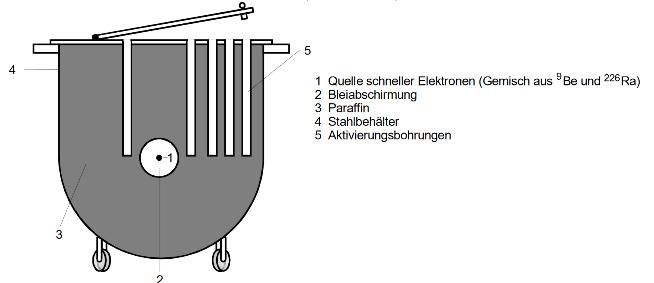
\includegraphics[scale=0.5]{Text/Bilder/neutronen.jpg}
\caption{Querschnitt durch die hier verwendete Quelle für thermische Neutronen \cite[213]{sample}}
\label{fig:ne}
\end{figure}

\subsection{Messung der Halbwertszeit}
Für die Anzahl der zum Zeitpunkt $t$ noch nicht zerfallenen Kerne gilt:
\begin{equation}
N(t)=N_0\mathrm{e}^{-\lambda t},\label{eq:N} \text{.}
\end{equation}
\begin{center}
  \small {($N_0 \: \hat{=} \: \text{Anzahl der Kerne zum Zeitpunkt $t=0$}$, $\lambda \: \hat{=} \: \text{Zerfallskonstante}$ )}
\end{center}
Aus \eqref{eq:N} folgt für die Halbwertszeit $\tau$:
\begin{equation}
\tau=\frac{\ln{(2)}}{\lambda} \text{.}\label{eq:T}
\end{equation}

Ebenso lassen sich mithilfe von \eqref{eq:N} die vorhandenen Kerne durch
\begin{equation}
  N_0-N(t)=N_\text{\Delta t}(t)=N_0\left(1-\mathrm{e}^{-\lambda \Delta t}\right)\mathrm{e}^{-\lambda t} \label{eqn:müde}
\end{equation}
bestimmen.
Der Ausdruck aus \eqref{eqn:müde} lässt sich zu dem linearen Zusammenhang
\begin{equation}
\ln{\left(N_\text{\Delta t}(t)\right)} = \ln{\left(N_0\left(1-\mathrm{e}^{-\lambda \Delta t}\right)\right)}-\lambda t \label{eqn:ln}
\end{equation}
umformen.
Werden geeignete Zeitintervalle gewählt und statistische und systematische Fehler somit gering gehalten, lassen sich mithilfe von \eqref{eqn:ln} die Zerfälle vieler Elemente untersuchen.

\subsection{Zerfallsreihen radioaktiver Isotope}
Beim Zerfall einiger Elemente, wie etwa Brom, ist lediglich ein Zerfallsprozess möglich.
Im Falle des Broms lautet dieser:
\begin{equation}
 \ce{^{79}_{35}Br} + \ce{^{1}_{0}n} \rightarrow \ce{^{80}_{35}Br} \rightarrow \ce{^{80}_{36}Kr} +  \beta^- + \bar{\nu}_\text{e} \text{.}
\end{equation}

Bei anderen Elementen, wie etwa Rhodium, sind jedoch mehrere Zerfälle möglich. Dieser Fall wird im folgendem diskutiert:
Wird $\ce{^{103}_{45}Rh}$ mit Neutronen beschossen, kann dieses zunächst zu einem angeregten Zwischenkern $\ce{^{104}_{45}Rh}$ wechseln um anschließend weiter zu zerfallen.
Die Wahrscheinlichkeit dafür liegt bei $10\%$.
Die andere, weitaus wahrscheinlichere Möglichkeit ist, dass der Zwischenkern keinen erhöhten Energiezustand annimmt, sondern direkt weiter zerfällt. Die Wahrscheinlichkeit dafür liegt bei $90\%$.
\begin{equation}
\ce{^{103}_{45}Rh} + \ce{^{1}_{0}n}
\begin{cases}
\underrightarrow{10\%}\ce{^{104i}_{45}Rh}\rightarrow \ce{^{104}_{45}Rh}+ \gamma \rightarrow \ce{^{104}_{45}Pd} + \beta^- + \symup{\bar{\nu}}_e \\
\underrightarrow{90\%}\ce{^{104}_{45}Rh}\rightarrow \ce{^{104}_{45}Pd} + \beta^- + \symup{\bar{\nu}}_e
\end{cases}
\end{equation}
Beide Zerfälle finden gleichzeitig statt, verfügen jedoch über unterschiedliche Halbwertszeiten.
Aufgrund der sehr kurzen Halbwertszeit $\tau$ ist die Aktivität von $\ce{^{104}_{45}Rh}$ zu Beginn der Messung sehr hoch.
Da hier jedoch, wie bereits erwähnt, unterschiedliche Zerfälle gleichzeitig stattfinden, kann die Halbwertszeit $\tau$ nicht exakt bestimmt werden.
